The system should be considered as stiff.

We decided to use linearised representation of systems in form of \eqref{governing_dis}, to find linearised matrix ${\bf A}^{(f)}(\bf F)$ and then compute the ratio of largest and smallest eigenvalue in matrix  ${\bf A}^{(f)}(\bf F)$. While the this operation was straightforward for $w$ and $U$ system, for $\Omega$ variable we decided to measure stiffens on $\Omega$ with the boundary condition \eqref{omega_boundary_1}, and also consider another case $\Omega_{(2)}$ where we use spline to approximate derivative and therefore have three non zero terms in first row of matrix  ${\bf A}^{(f)}(\bf F)$, instead of just one term as the consequence form direct usage of \eqref{omega_boundary_1}. We have computed so defined stiffness for all six benchmarks cases (Appendix \ref{app:A}) and both mesh options \eqref{mesh_uniform} and \eqref{mesh_power}. It would be however to much to present all that data in this paper, therefore we would like to highlight the most interesting points.
First let us plot eigenvalues ratio computed for up to $N=1000$ with fixed $\epsilon=10^{-2}$ for benchmark with Carter type leak off:

\begin{figure*}
        \begin{subfigure}[b]{0.33\textwidth}
                \centering
                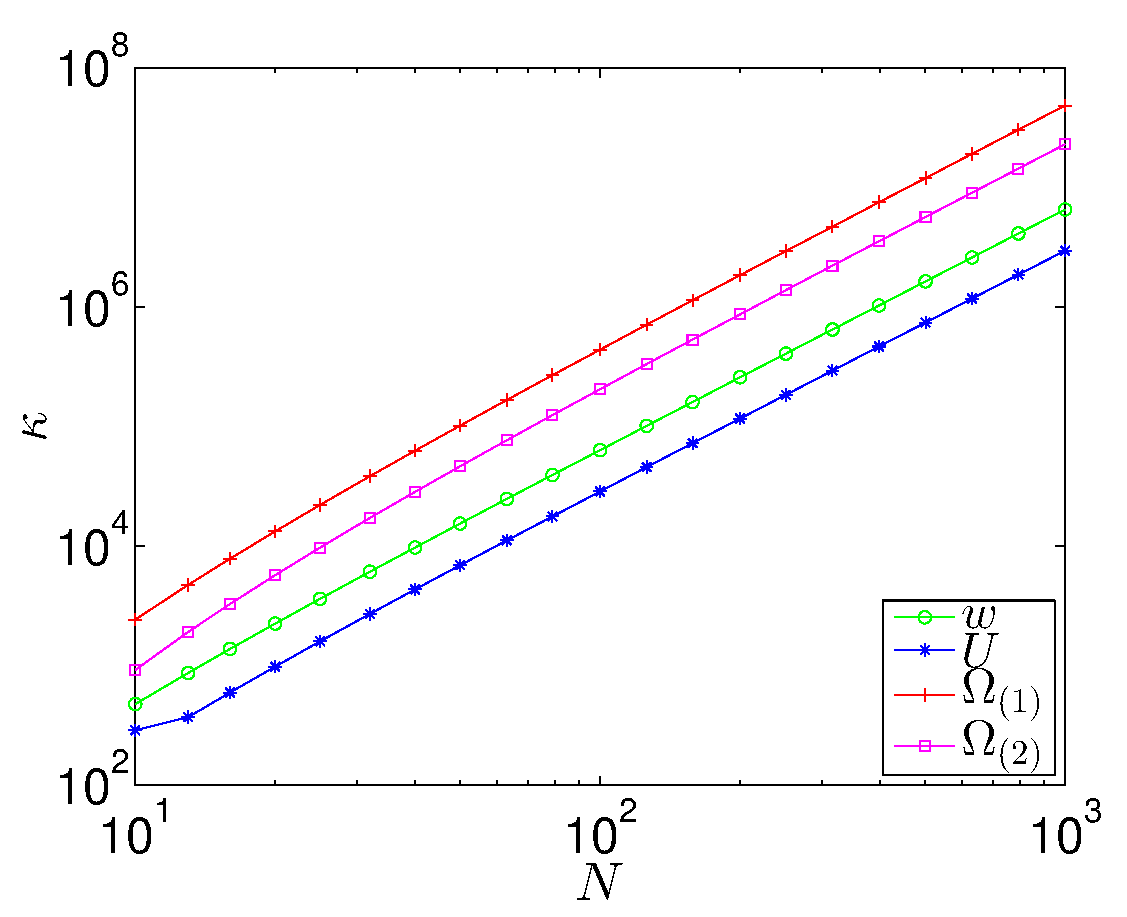
\includegraphics[width=\textwidth]{3_PKN_numerical/stiffness/stiff_carter3.eps}
                \caption{ratio $Q_l/q_0=0.9$ on $x_m^{(1)}$ mesh}
                \label{s_plot3}
        \end{subfigure}
        \begin{subfigure}[b]{0.33\textwidth}
                \centering
                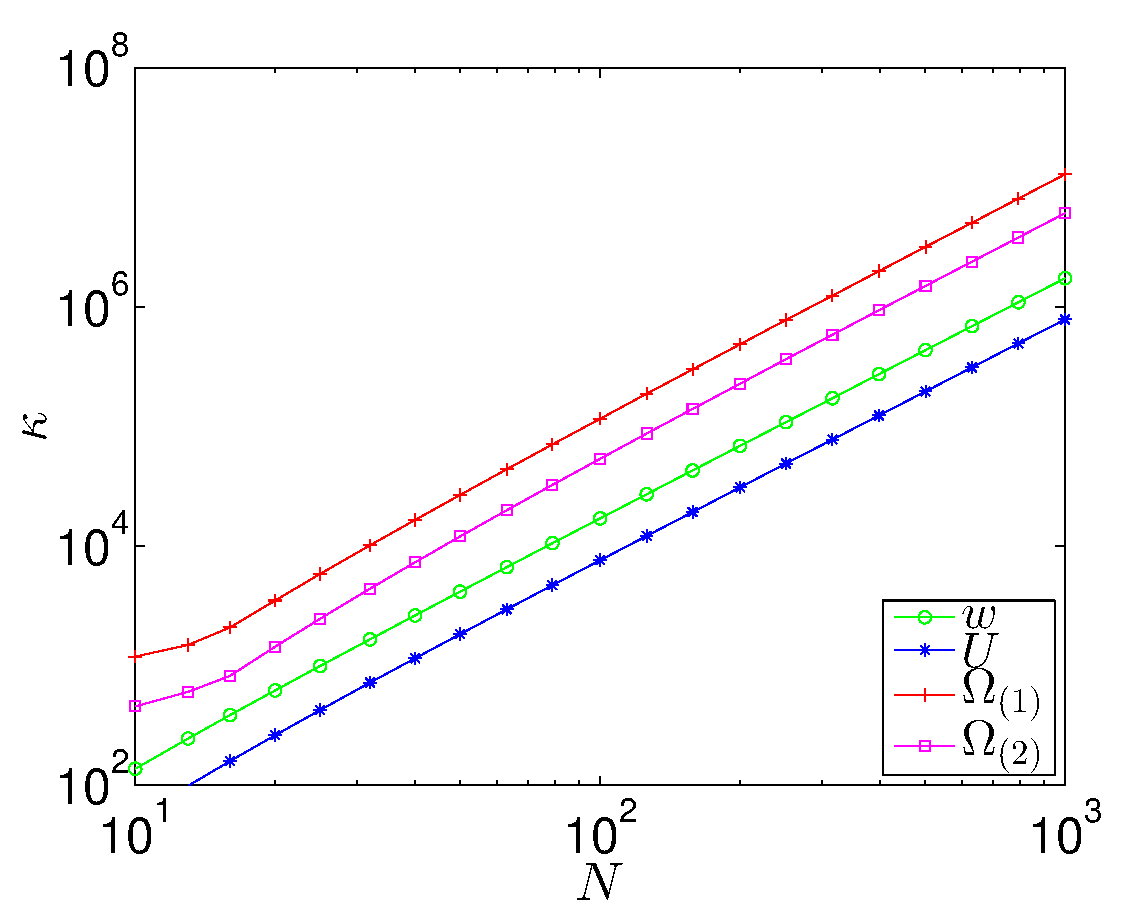
\includegraphics[width=\textwidth]{3_PKN_numerical/stiffness/stiff_carter1.eps}
                \caption{ratio $Q_l/q_0=0.9$ on $x_m^{(2)}$ mesh }
                \label{s_plot1}
        \end{subfigure}
        \begin{subfigure}[b]{0.33\textwidth}
                \centering
                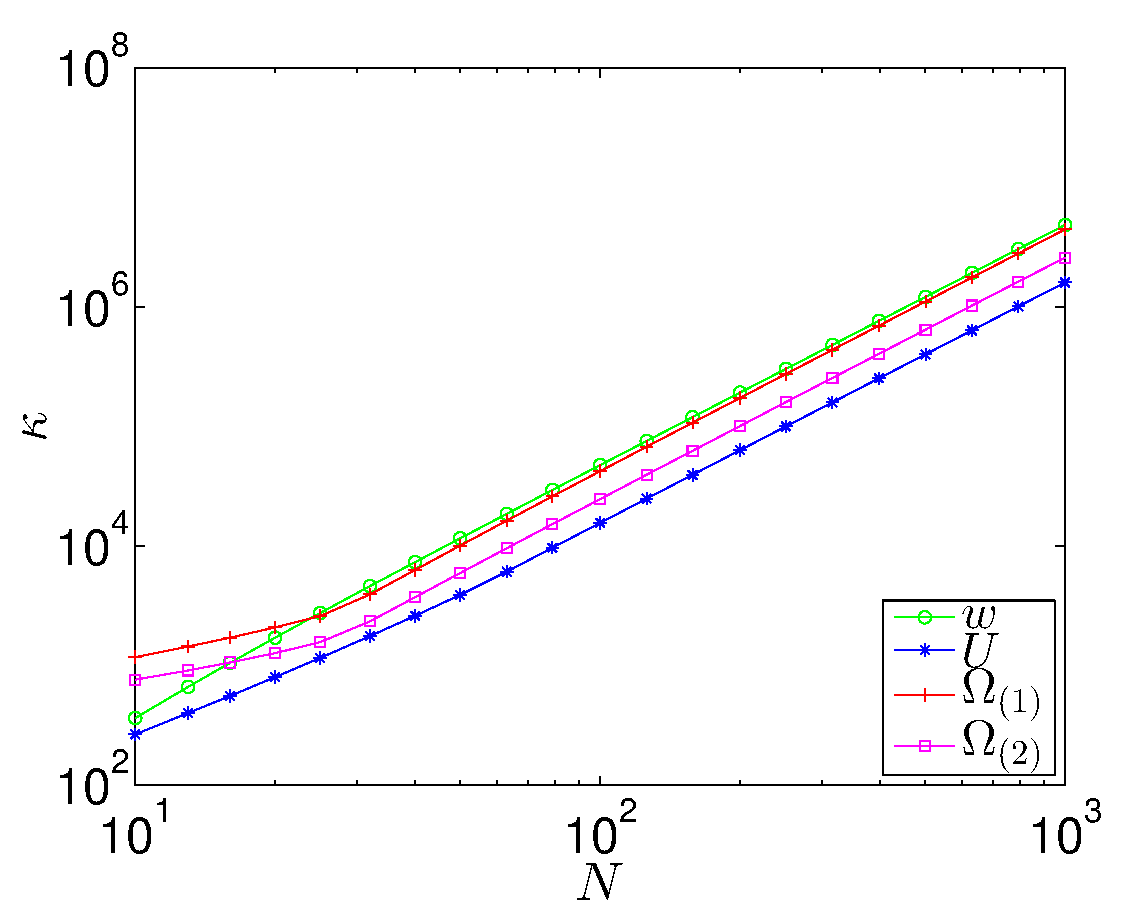
\includegraphics[width=\textwidth]{3_PKN_numerical/stiffness/stiff_carter2.eps}
                \caption{ratio $Q_l/q_0=0.5$ on $x_m^{(2)}$ mesh }
                \label{s_plot2}
        \end{subfigure}
\caption{Stiffness in logarithmic scale defined as ratio of smallest and largest eigenvalue in linearised matrix  ${\bf A}^{(f)}(\bf F)$ ($\epsilon=10^{-3}$)}
\label{fig:stiffness_a}
\end{figure*}

As we can see on Figure \ref{fig:stiffness_a}, the least stiff formulation is $U$, and that result repeats in all of tests we concluded. However if $w$ should be considered stiffer than $\Omega$ formulation is depends on the benchmark type. The change of ratio form 1:1 seems to have negative effect on $w$ system and positive effect on $\Omega$. The boundary condition \eqref{omega_boundary_1} also has a negative effect on stiffness of $\Omega$ and can be replaced by  some other three point based condition (and that change had appeared to have no consequences on accuracy of our tests).  Stiffness of all of the systems can be fairly approximated as $AN^2$ as it is clear that straight lines are plotted on logarithmic scales, however that approximation only is valid for values of about $\epsilon>\frac{1}{N^2}$. With very small epsilons and insufficiently large $N$ there is a different trend in stiffness. See the Figure \ref{s_plot3} for a plot of this phenomena.

\begin{figure}
\centering
        \begin{subfigure}[b]{0.48\textwidth}
                \centering
                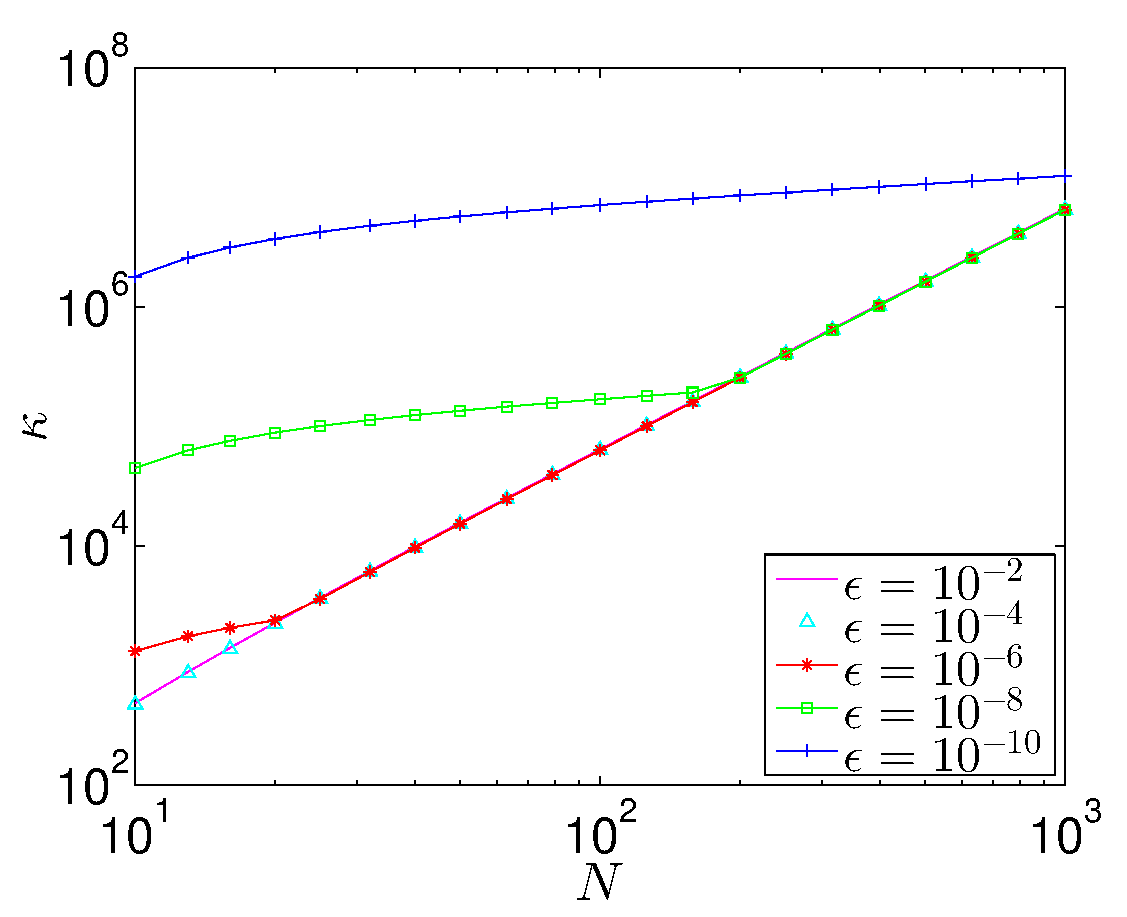
\includegraphics[width=\textwidth]{3_PKN_numerical/stiffness/stiff_epsilons_1.eps}
                \caption{Stiffness for $w$ system compared against various $\epsilon$ values on uniform grid, there are two stiffness behaviours depending on the choice of $N$ relative to $\epsilon$}
                \label{s_plot5}
        \end{subfigure}
        \begin{subfigure}[b]{0.48\textwidth}
                \centering
                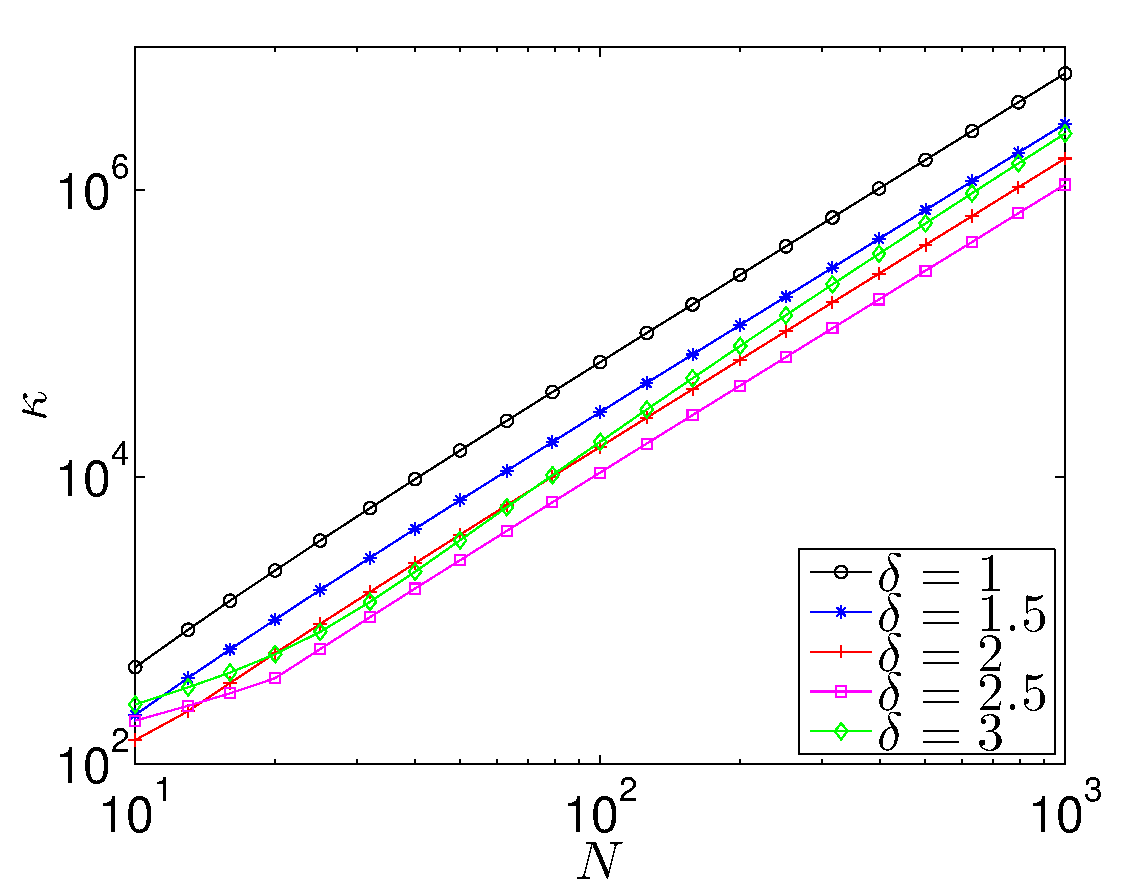
\includegraphics[width=\textwidth]{3_PKN_numerical/stiffness/y_vs_uniform.eps}
                \caption{Stiffness for $w$ system with  $x^{(2)}_m$ mesh \eqref{mesh_power} for various $\delta$ values, result obtained on unform mesh \eqref{mesh_uniform} would overlap $\delta=1$}
                \label{s_plot6}
        \end{subfigure}
\caption{Effects of different values of $\epsilon$ and $\delta$ on stiffness (TAK WYCHODZI NA TO ZE JEDNAK 2 NIE JEST OPTYMALNE) }
\label{fig:stiffness_b}
\end{figure}

The choice of spacial discretization between uniform  $x^{(1)}_m$  mesh \eqref{mesh_uniform} and $x^{(2)}_m$  mesh \eqref{mesh_power} has an effect of stiffness. As we predicted in [???,MWL] the $x^{(2)}_m$  mesh improves system stiffness for about an order of magnitude compared to uniform mesh, when the optimal value of $\delta=2$ is chosen. However that point is valid only for if the condition $\epsilon>\frac{1}{N^2}$ is fulfilled. For small values of $N$ a choice of smaller $\delta$ value may be beneficial.

PONIZEJ TAK BYLO DLA OMEGI, ALE NIE WIEM CZY TO BEDIE DALEJ POTRZEBNE

On Figure \ref{s_plot4} we can see that indeed for $N>100$ and fixed $\epsilon=10^{-4}$ the $x^{(2)}_m$  mesh has lowest stiffness for the optimal value of $\delta=2$. With the values of $N<100$ the optimal value of $\delta$ gets smaller, to eventually reach $\delta=1$ for ten points mesh $N=10$. If the condition $\epsilon>\frac{1}{N^2}$ is not meet it is a better choice from the point of minimizing stiffness to use values of $\delta$ smaller than the otherwise optimal $2$.

\begin{table}
\centering
\begin{tabular}{c| c@{}|c@{}|c@{}|c@{}|c@{}|c@{}|}
\cline{2-7}
& \multicolumn{3}{c|}{$Q_l/q_l=0.9$} & \multicolumn{3}{c|}{$Q_l/q_l=0.5$} \\ \cline{2-7}
& $q_l^{(1)}$ & $q_l^{(2)}$ & $q_l^{(3)}$ & $q_l^{(1)}$ & $q_l^{(2)}$ & $q_l^{(3)}$\\ \cline{2-7}
& \multicolumn{6}{c|}{A values for $w$ }\\ \cline{1-7}
\multicolumn{1}{|c|}{$x_m^{(1)}$} 
&6.5e+0&6.6e+0&6.8e+0&1.8e+1&1.8e+1&1.8e+1 \\ \cline{1-7} \multicolumn{1}{|c|}{$x_m^{(2)}$}
&1.7e+0&1.7e+0&1.7e+0&4.6e+0&4.7e+0&4.7e+0
  \\ \cline{1-7}
& \multicolumn{6}{c|}{A values for $U$ }\\ \cline{1-7}
\multicolumn{1}{|c|}{$x_m^{(1)}$} &3.0e+0&3.0e+0&3.2e+0&6.0e+0&6.1e+0&6.2e+0 \\ \cline{1-7} \multicolumn{1}{|c|}{$x_m^{(2)}$}
&7.5e-1&7.7e-1&8.1e-1&1.5e+0&1.5e+0&1.6e+0
  \\ \cline{1-7}
& \multicolumn{6}{c|}{A values for $\Omega_{(1)}$ }\\ \cline{1-7}
\multicolumn{1}{|c|}{$x_m^{(1)}$} 
&4.8e+1&4.8e+1&4.9e+1&1.7e+1&1.7e+1&1.7e+1 \\ \cline{1-7} \multicolumn{1}{|c|}{$x_m^{(2)}$}
&1.2e+1&1.2e+1&1.3e+1&4.3e+0&4.3e+0&4.3e+0
  \\ \cline{1-7}
& \multicolumn{6}{c|}{A values for $\Omega_{(2)}$ }\\ \cline{1-7}
\multicolumn{1}{|c|}{$x_m^{(1)}$} 
&2.3e+1&2.2e+1&1.9e+1&9.6e+0&1.0e+1&1.3e+1 \\ \cline{1-7} \multicolumn{1}{|c|}{$x_m^{(2)}$}
&5.8e+0&5.7e+0&4.7e+0&2.5e+0&2.6e+0&3.5e+0
  \\ \cline{1-7}
\end{tabular}
\caption{Values of $A$ form aproximation $AN^2$ at $N=1000$ and $\epsilon=10^{-4}$ ($\delta=2$ for $x_m^{(2)}$ mesh)}
\label{table_A}
\end{table}

In our analysis, we quantify the system stiffness by a condition
ratio $\kappa_A$ defined in (\ref{kappa}).
Since the problem is nonlinear, our
investigation is to be done for the linearized form of matrix ${\bf
A}^{(f)}$. It is obvious that for all six variants of benchmark
solutions under consideration (see Appendix \ref{app:A}) one has
different values of ${\bf A}^{(f)}$. Computations are carried out
for two types of meshes (the uniform and non-uniform one). For each
of the benchmark solutions, one obtains a constant  value for the condition ratio (independent on
time), apart from the fact that the matrix
 ${\bf A}^{(f)}$ depends on time. Those values of the condition ratio $\kappa_A$ are,
generally speaking, different for
various benchmarks and chosen meshes.

Before comparing the results for various dependent variables, we
have checked that for the dynamic system based on $U$ the stiffness
is almost identical for both forms of the regularized boundary
condition at $x=1-\varepsilon$ ((\ref{L3}) and (\ref{BC_N})
respectively). Thus, for the rest of the dependent variables ($w$ and
$\Omega$) we restrict our stiffness investigation only to the
formulation (\ref{BC_N}). Remarkably, the situation changes
dramatically when one considers the accuracy of  computations, which
shall be discussed later on.

Computing the condition ratio for the next variants of the matrix
linearization, we have confirmed the following estimate valid for large values of
$N$ for all cases under investigation:
\begin{equation}
\label{kappa}
\kappa_A^{(f)}=\frac{|\lambda_{max}|}{|\lambda_{min}|}\sim \varpi^{(f)} N^2,\quad N\to\infty.
\end{equation}
Here $|\lambda_{max}|$, and $|\lambda_{min}|$ are the largest and
smallest absolute values among the ${\bf A}^{(f)}$ matrix
eigenvalues, while the constant $\varpi^{(f)}$ is to be estimated
numerically. Its values for all six benchmark cases are shown in
 Table~\ref{table_A}.


Although the qualitative character
of the stiffness behaviour ($N^2$) is rather obvious, its
quantitative measure described by $\varpi$ can be used to select the
optimal (in terms of the stiffness properties) variant of the
dynamic system.


\begin{table}[h*]
\centering
\begin{tabular}{c| c@{}|c@{}|c@{}|c@{}|c@{}|c@{}|}
\cline{2-7}
& \multicolumn{3}{c|}{$Q_l/q_0=0.9$} & \multicolumn{3}{c|}{$Q_l/q_0=0.5$} \\ \cline{2-7}
& $q_l^{(1)}$ & $q_l^{(2)}$ & $q_l^{(3)}$ & $q_l^{(1)}$ & $q_l^{(2)}$ & $q_l^{(3)}$\\ \cline{2-7}
& \multicolumn{6}{c|}{$\varpi$ estimated for the system based on variable $w$}\\ \cline{1-7}
\multicolumn{1}{|c|}{$x^{(I)}$}
&6.5e+0&6.6e+0&6.8e+0&1.8e+1&1.8e+1&1.8e+1 \\ \cline{1-7} \multicolumn{1}{|c|}{$x^{(II)}$}
&1.7e+0&1.7e+0&1.7e+0&4.6e+0&4.7e+0&4.7e+0
  \\ \cline{1-7}
& \multicolumn{6}{c|}{$\varpi$ estimated for the system based on variable $U$ }\\ \cline{1-7}
\multicolumn{1}{|c|}{$x^{(I)}$} &3.0e+0&3.0e+0&3.2e+0&6.0e+0&6.1e+0&6.2e+0 \\ \cline{1-7} \multicolumn{1}{|c|}{$x^{(II)}$}
&7.5e-1&7.7e-1&8.1e-1&1.5e+0&1.5e+0&1.6e+0
  \\ \cline{1-7}
& \multicolumn{6}{c|}{$\varpi$ estimated for $\Omega_{(1)}$ based on  condition (\ref{omega_boundary_1})}\\ \cline{1-7}
\multicolumn{1}{|c|}{$x^{(I)}$}
&4.8e+1&4.8e+1&4.9e+1&1.7e+1&1.7e+1&1.7e+1 \\ \cline{1-7} \multicolumn{1}{|c|}{$x^{(II)}$}
&1.2e+1&1.2e+1&1.3e+1&4.3e+0&4.3e+0&4.3e+0
  \\ \cline{1-7}
& \multicolumn{6}{c|}{$\varpi$ estimated for $\Omega_{(2)}$ based on condition (\ref{BC_0})}\\ \cline{1-7}
\multicolumn{1}{|c|}{$x^{(I)}$}
&2.3e+1&2.2e+1&1.9e+1&9.6e+0&1.0e+1&1.3e+1 \\ \cline{1-7} \multicolumn{1}{|c|}{$x^{(II)}$}
&5.8e+0&5.7e+0&4.7e+0&2.5e+0&2.6e+0&3.5e+0
  \\ \cline{1-7}
\end{tabular}
\caption{Values of the parameter $\varpi^{(f)}$ from the
approximation of the condition ratio (\ref{kappa}) for the different
dynamic systems (\ref{governing_dis}) and different benchmarks. The computations were provided for $\varepsilon =10^{-3}$} \label{table_A}
\end{table}

\vspace{-4mm}

The following analysis includes investigation of stiffness
sensitivity to: i) the solution (benchmark) type, ii) choice of the
dependent variable, iii) choice of the independent variable
(spatial mesh), iv) value of the regularization parameter
$\varepsilon$.




{\sc Remark 5.} As mentioned previously, in case of the variable
$\Omega$, there are two alternative ways to introduce the boundary
condition at $x=0$ to the system -formulations
(\ref{omega_boundary_1}) and (\ref{BC_0}), respectively. In this way
one can construct two alternative dynamic systems of different
dimensions ($N$ and $N-1$). The results  in Table~\ref{table_A} show
that the stiffness properties of the system corresponding to the
boundary condition (\ref{BC_0}) are slightly better than those of
the system utilizing (\ref{omega_boundary_1}). Indeed, the
respective parameter $\varpi$ is about two times smaller. One of the
possible explanations is the aforementioned difference in the
systems' sizes: $\dim {\bf A}^{(\Omega)}_{(1)}=\dim {\bf
A}^{(\Omega)}_{(2)}+1$ (see Remark 3). We have checked that the
accuracy of computations remains practically the same regardless of
the system variant. Taking this fact into account, we restrict
ourselves in the analysis only to the system which employs the
boundary condition at point $x=0$ in the form (\ref{BC_0}). Thus,
from now on all the investigated dynamic systems (for all dependent
variables) will be based on the same mechanisms for incorporation of
the boundary conditions.



\begin{figure}[h*]
\centering
        \begin{subfigure}[b]{0.35\textwidth}
                \centering
                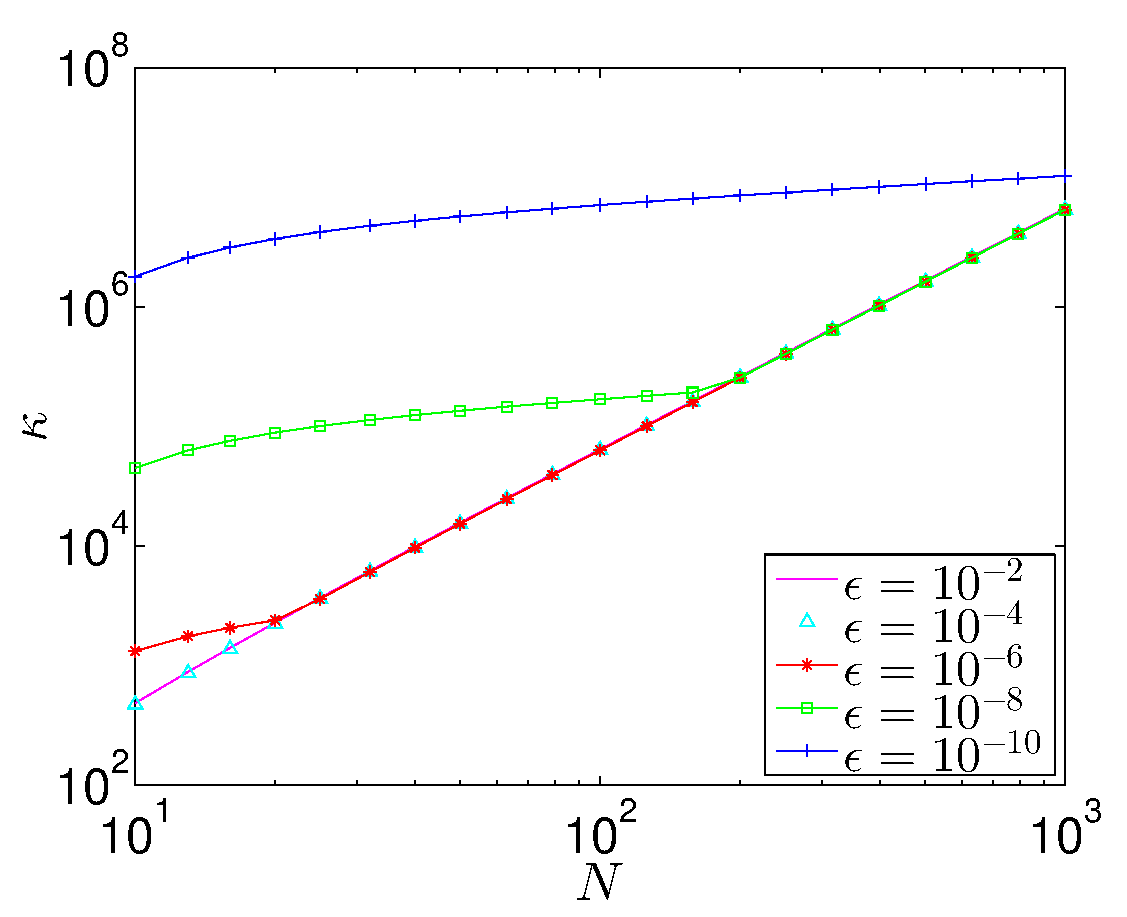
\includegraphics[width=\textwidth]{3_PKN_numerical/stiffness/stiff_epsilons_1.eps}
                \begin{picture}(0,0)(85,-117)
        \put(50,-80){$Q_l/q_0=0.9$}
        \put(5,-35){$\kappa$}
        \put(82,-110){$N$}
        \end{picture}

        \end{subfigure}

\vspace{-2mm}

\caption{Condition ratio $\kappa=\kappa^{(w)}(N)$ for the dynamic system based on $w$ variable and different values of the regularization parameter $\varepsilon$.
The case of the uniform mesh is analyzed.}
\label{fig:stiffness_b}
\end{figure}



Influence of the value of $\varepsilon$ on the condition ratio is analyzed in Fig.~\ref{fig:stiffness_b}.
As an example, we present here the benchmark $q_l^{(1)}$ for $Q_l/q_0=0.9$ (see Appendix C).
The results were obtained for the uniform mesh.
For other combinations of the benchmark solutions and different meshes the graphs have
similar character.
As anticipated, the estimation \eqref{kappa}  holds true
only for sufficiently large $N$.
The threshold value of $N$ depends
on the chosen $\varepsilon$.
Thus for a fixed number of grid
points $N$, there is a critical value of the regularization parameter
$\varepsilon_s(N)$ for which the stiffness characteristics changes its behaviour.
 By
taking $\varepsilon<\varepsilon_s(N)$ one increases appreciably the system
stiffness.


The results of the stiffness investigation are collected in the
Table~\ref{table_A} and Fig.~\ref{fig:stiffness_b} The following
conclusions can be drawn from this data:






\begin{itemize}
\item [(i)] The nonuniform mesh reduces the stiffness approximately up to five times
regardless of the solution type (Table~\ref{table_A});

\item [(ii)] The most important parameter affecting the stiffness properties is the relation between
the injection flux rate and the leak-off to the formation $Q_l/q_0$ as can be clearly seen in
Table~\ref{table_A}. The value of this parameter is more important
than a particular distribution of the leak-off function (and its behaviour near the crack tip);


\item [(iii)] When comparing systems for various dependent variables,
the lowest condition ratio gives the system built for $U$ (one
order of magnitude lower than the others). The worst
stiffness performance takes place for the system corresponding to the
$\Omega$-variable. However, in some cases $\Omega$ may produce lower stiffness than $w$;

\item [(v)] A value of the regularization parameter $\varepsilon$
essentially affects  the stiffness of a dynamic system.
\end{itemize}